\begin{frame}[plain]
  \begin{figure}
    \centering
    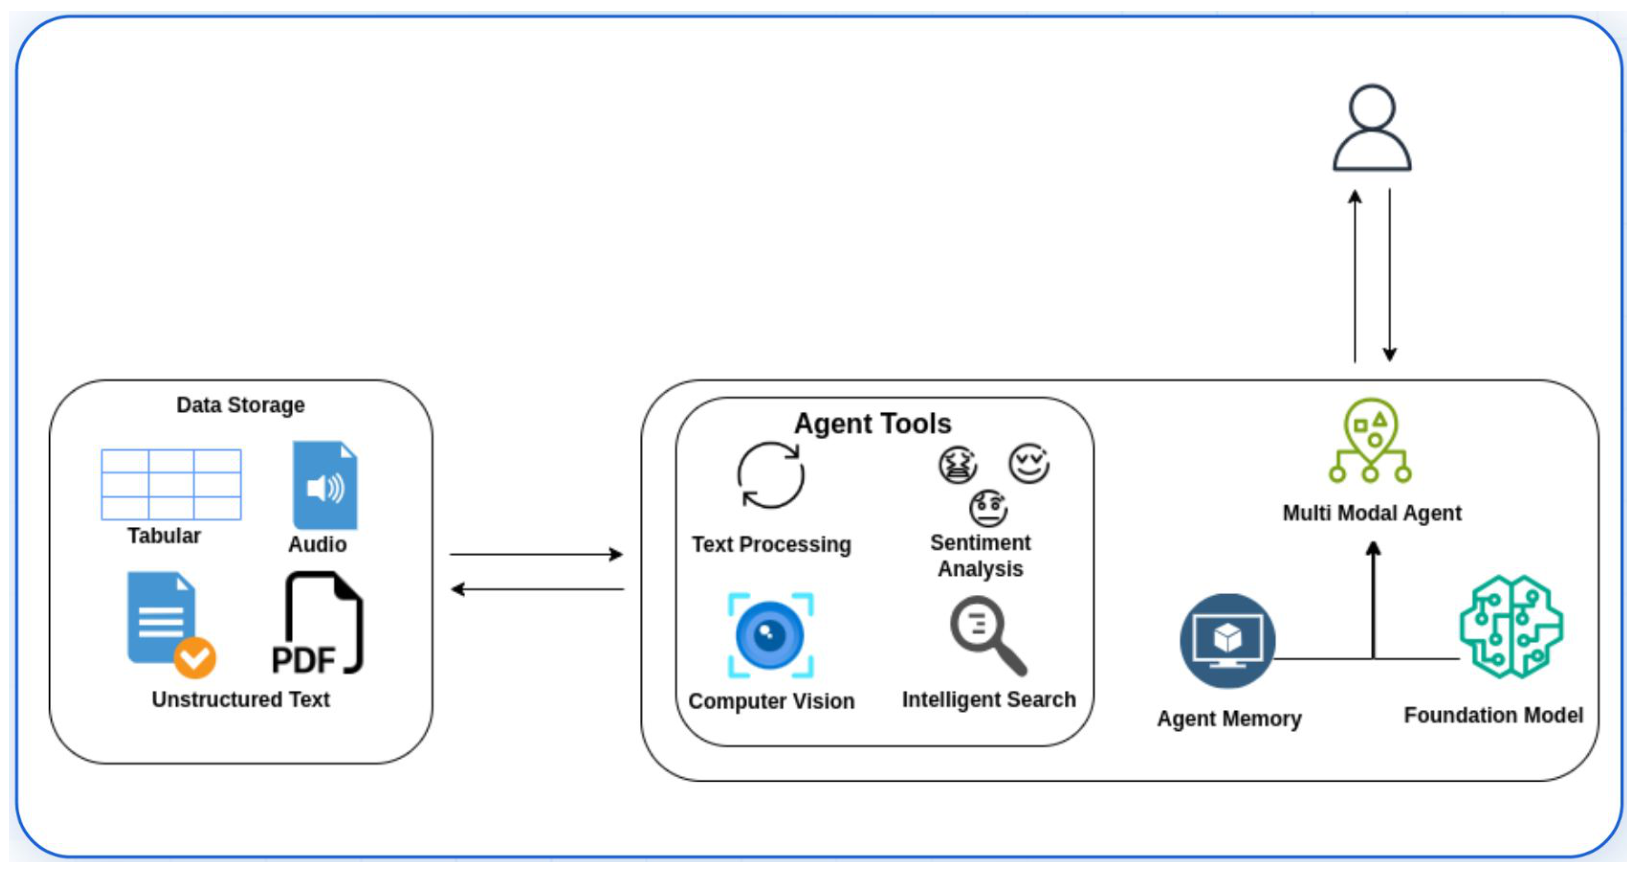
\includegraphics[width=0.8\paperwidth,height=0.74\paperheight,keepaspectratio]{images/multimodal-nlp-agentic-ai/multimodal_agent_system_overview.png}
    \caption*{\scriptsize Redrawn after Nath et al., ``Generative AI and multi-modal agents in AWS: The key
    to unlocking new value in financial markets'', AWS Machine Learning Blog, 2023 (``Architecture Pattern:
    Multi-modal Agent'').}
  \end{figure}
\end{frame}

\begin{frame}{Table of Contents}
  \begin{enumerate}
    \item Motivation
    \item Learning Outcomes
    \item Vision-Language Models
      \begin{enumerate}
        \item CLIP: Contrastive Language-Image Pretraining
        \item VisualBERT and the Visual BERT family
        \item FLAVA, and on to multimodal LLMs
      \end{enumerate}
    \item Multimodal Architectures
      \begin{enumerate}
        \item Categories of Multimodal Architectures
        \item Challenges in Multimodal Integration
      \end{enumerate}
    \item Agentic AI
      \begin{enumerate}
        \item What is Agentic AI?
        \item Reactive vs. Proactive Agents
      \end{enumerate}
  \end{enumerate}
\end{frame}

\begin{frame}{Table of Contents (contd.)}
  \begin{enumerate}
    \setcounter{enumi}{5}
    \item Agent Loop, Tool Use, and Agentic RAG
    \item Open-Source Agentic Frameworks
      \begin{enumerate}
        \item Auto-GPT
        \item BabyAGI
        \item Other Notable Frameworks
      \end{enumerate}
    \item Continual Learning in Agents
      \begin{enumerate}
        \item Why Continual Learning?
        \item Challenges in Continual Learning
      \end{enumerate}
    \item Safety, Ethics, and Control
      \begin{enumerate}
        \item Safety in Agentic Systems
        \item Ethics and Control
      \end{enumerate}
    \item Future Directions
  \end{enumerate}
\end{frame}
